\chapter{Chromatic Page:}
The PTC page, also known as the Chromatic Page, is used to play MD tracks chromatically using the MD Trigger interface or an attached MIDI Keyboard.

\screenshot{chroma.png}

For supported track types, the Track’s Pitch is mapped to Notes of a selected scale across the MD Trigger interface.

Melodies can be recorded in real-time.


%\fbox{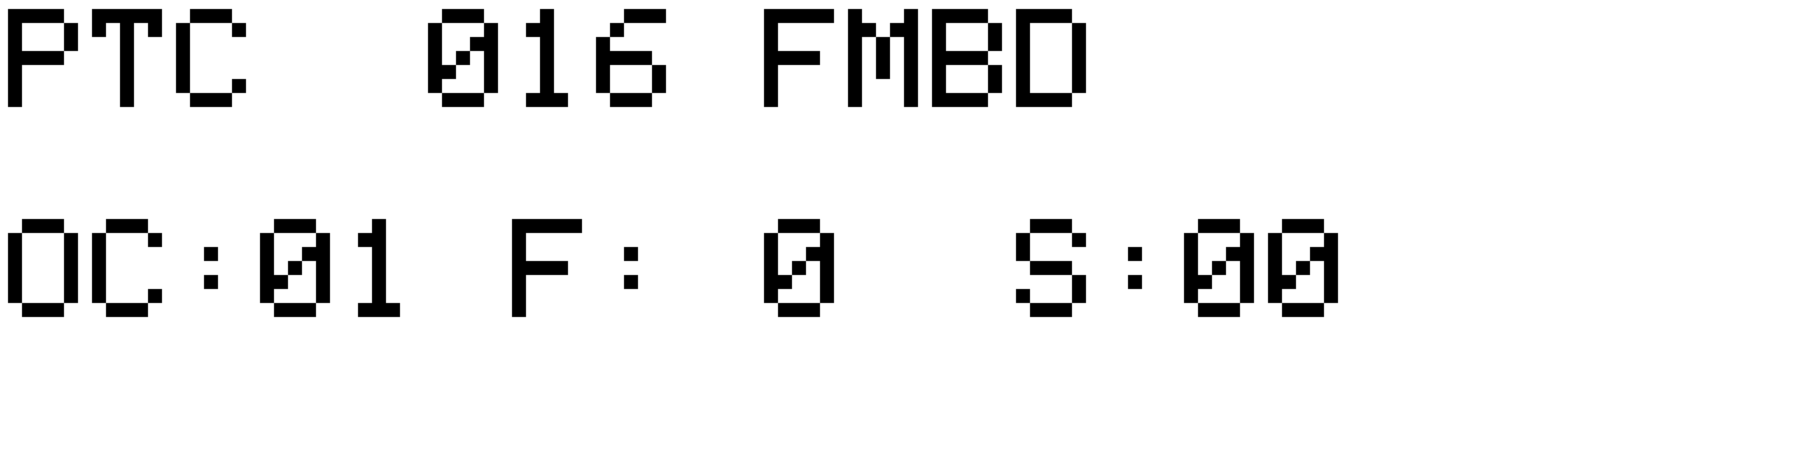
\includegraphics[scale=.40]{ptc_md.png}}\\\\



\textit{To enter the PTC Page: Select desired track on MD by pressing \textbf{[ Function ] + [ Track N ]}. Enter the PTC mode by pressing \textbf{[Shift1|PageSelect]} and \textbf{[Trigger 8] }.}

\screenshot{chromat_action.png}

\textit{A keyboard will be displayed showing the current active notes.}
\\

\encodersbuttons{Octave (OC)}{Fine Tune (F)}{Track Length}{Scale Type (S)}{Toggle PTC/RPTC}{PageSelect}{Clear Track}{Track/Trig Menu}
	
\section{A4 + ExtMIDI:}
The PTC Page is also used to record/play the Analog4 or ExtMIDI tracks. Scale modes are also supported for these track types.\\

\section{Recording a sequence:}
\textit{Press the \textbf{[ Save ] }button to enable record mode, RPTC.\\}

Play notes on either the MD or A4/ExtMidi to record a melody.

\vspace{-0.3cm}

\section{Clearing recorded sequence:}
\begin{itemize}
\item To clear the current track, press and hold the\textbf{ [ Shift2 ]} to open the track menu, rotate \textbf{[Encoder2]} to the entry \textbf{CLEAR}, then rotate \textbf{[Encoder1]} to select \textbf{TRK}.
\item To clear all tracks of the current track type, select \textbf{ALL}.
\item The current track can also be quickly cleared by pressing \textbf{[Write]}.
\end{itemize}


\vspace{-0.3cm}

\section{Changing track length:}
\begin{itemize}
\item Track length is controlled by rotating \textbf{[ Encoder 3 ]}.
\item To change the lengths of all tracks of the current track type, simultaneously hold down \textbf{[Write]} whilst rotating \textbf{[ Encoder 3 ]}.
\item Track length can also be set by holding \textbf{[Write]} and then selecting the corresponding step from the MD trigger interface. The track length is offset by the current track-page.
\end{itemize}


\section{A4 or ExtMidi}
Melodies and chords can be played and recorded from the Analog4 or ExtMIDI device in the PTC and RPTC pages.
\\

If using the Analog 4, select the desired track using the A4’s track select buttons. The first note played on the mini keyboard will cause the PolyStep edit page to switch to  the corresponding external sequencer track.
\\

\textit{The active device tab will switch over from MD to A4/MI, in the left information panel, when such midi notes are received.}
\\

Switching Between Low and High Resolution Modes on Poly Sequencer Tracks.
Press \textbf{[Shift2]} then rotate \textbf{[Encoder2]} to select the \textbf{TRACK RES.} entry.
